\begin{center}
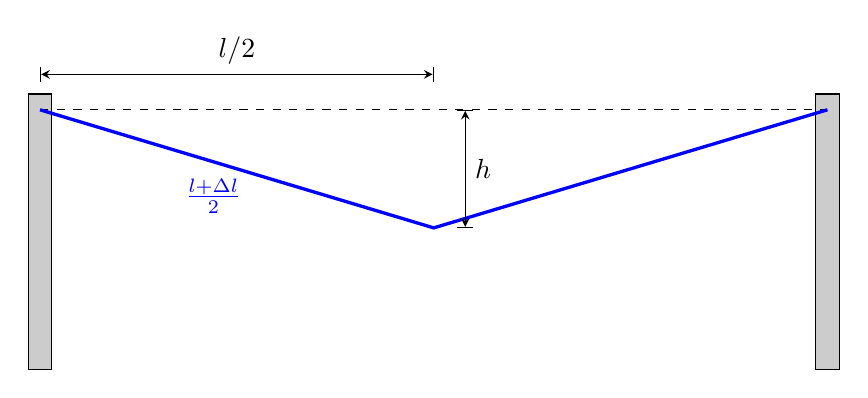
\begin{tikzpicture}[>=stealth]
 \fill[gray!40] (-0.15,0) rectangle (0.15,3.5);
 \fill[gray!40] (9.85,0) rectangle (10.15,3.5);
 \draw (-0.15,0) rectangle (0.15,3.5);
 \draw (9.85,0) rectangle (10.15,3.5);
 \draw[dashed] (0,3.3) -- (10,3.3);
 \draw[very thick, blue] (0,3.3) -- (5,1.8) -- (10,3.3);
 \draw[|<->|] (5.4,3.3) -- (5.4,1.8) node[midway, right] {$h$};
 \draw[|<->|] (0,3.75) -- (5,3.75) node[midway, above] {$l/2$};
 \node[blue] at (2.2,2.2) {$\frac{l+\Delta l}{2}$};
\end{tikzpicture}
\end{center}

Annahme: An einem heissen Sommertag hat die Leitung in der Sonne etwa \THeO. Die Temperaturdifferenz ist $\Delta\vartheta = \dTsF = \dTs$. Mit $\alpha = \alAlO$ (Aluminium, FoTaBe S.~190) wird die Leitung länger um
\begin{align}
 \Delta l &= \dlLF = \alAl\cdot\lMa\cdot\dTs = \dlL
\end{align}
Nähert man die durchhängende Leitung durch zwei gerade Stücke der Länge $(l+\Delta l)/2$ an, folgt der Durchhang $h$ in der Mitte aus dem Satz von Pythagoras:
\begin{align}
 h &= \hDuF \\
   &= \sqrt{\left(\frac{\lMa+\dlL}{2}\right)^2-\left(\frac{\lMa}{2}\right)^2} \\
   &= \hDu \approx \result{\hDuP{0}{1}}
\end{align}
Eine Verlängerung um nur zwei Promille führt also zu einem Durchhang von einigen Metern.
